\documentclass[11pt, a4paper, oneside]{Thesis}
\usepackage{floatrow}
\floatsetup[table]{capposition=top}
\usepackage{xurl}
\usepackage{textcomp}
\usepackage{wrapfig}
\usepackage{pdfpages}
\usepackage{lscape}
\usepackage{rotating}
\usepackage{graphicx}
\usepackage{seqsplit}
\usepackage{enumerate}
\usepackage{amsmath}
\usepackage{upgreek}
\usepackage{url}
\usepackage{gensymb}
\usepackage{csquotes}
\usepackage{notoccite}
\usepackage{enumitem}
\usepackage{multirow}
\usepackage[font=small,skip=0.333\baselineskip]{caption}
\renewcommand{\chapterautorefname}{Chapter}
\usepackage{acronym}
\usepackage{array}
\newcolumntype{L}{>{\centering\arraybackslash}m{3cm}}

\makeatletter
\AtBeginDocument{%
  \renewcommand*{\AC@hyperlink}[2]{%
    \begingroup
      \hypersetup{hidelinks}%
      \hyperlink{#1}{#2}%
    \endgroup
  }%
}
\makeatother

\graphicspath{{figures/}{Pictures/}}
\usepackage[square, numbers]{natbib}
\hypersetup{urlcolor=black, colorlinks=true}
\title{\ttitle}

\begin{document}
% Oneside thesis: avoid blank verso pages from \cleardoublepage in the class file.
\let\cleardoublepage\clearpage

\makeatletter
\renewcommand*{\NAT@nmfmt}[1]{\textsc{#1}}
\makeatother

\frontmatter
\setstretch{1.6}
\fancyhead{}
\rhead{\thepage}
\lhead{}
\pagestyle{fancy}
\newcommand{\HRule}{\rule{\linewidth}{0.5mm}}

\hypersetup{pdftitle={\ttitle}}
\hypersetup{pdfsubject=\subjectname}
\hypersetup{pdfauthor=\authornames}
\hypersetup{pdfkeywords=\keywordnames}

%----------------------------------------------------------------------------------------
%	TITLE PAGE
%----------------------------------------------------------------------------------------
\begin{titlepage}
\begin{center}
\HRule \\[0.4cm]
{\huge \bfseries \ttitle}\\[0.4cm]
\HRule \\[1.5cm]
\large \textit{A thesis submitted in fulfilment of the requirements\\ for the degree of \degreename}\\[0.3cm]
\textit{by}\\[0.4cm]
\authornames \\ Roll No. \\
\vfill
to the\\
\DEPTNAME\\
\textsc{\UNIVNAME}\\[1.5cm]
\large \today\\[2cm]
\end{center}
\end{titlepage}

%----------------------------------------------------------------------------------------
%	DECLARATION PAGE
%----------------------------------------------------------------------------------------
\Declaration{\addtocontents{toc}{\vspace{1em}}}
\setcounter{page}{2}
\begin{minipage}{\textwidth}
It is certified that the work contained in this thesis entitled \textbf{\enquote{\ttitle}} by \textbf{\authornames} has been carried out under my supervision and that it has not been submitted elsewhere for a degree.
\end{minipage}
\vspace{20mm}
\begin{minipage}{0.49\textwidth}
\begin{flushleft}
{\supnameA\\
Professor\\
\deptname\\
\univname\\
\today}
\end{flushleft}
\end{minipage}

\StudentDeclaration{\addtocontents{toc}{\vspace{1em}}}
This is to certify that the thesis titled \textbf{``\ttitle''} has been authored by me. It presents the research conducted by me under the supervision of \textbf{\supnameA}.\par
To the best of my knowledge, it is an original work, both in terms of research content and narrative, and has not been submitted elsewhere, in part or in full, for a degree. Further, due credit has been attributed to the relevant state-of-the-art and collaborations with appropriate citations and acknowledgements, in line with established norms and practices.\\ [1cm]
\begin{minipage}{.5\textwidth}
\begin{flushleft}
{\authornames\\ Roll No. \\
\normalsize{\href{https://www.iitk.ac.in/ph/}{\deptname}\\
\univname}}
\end{flushleft}
\end{minipage}

%----------------------------------------------------------------------------------------
%	ABSTRACT PAGE
%----------------------------------------------------------------------------------------
\lhead{\emph{Abstract}}
\abstract{\addtocontents{toc}{\vspace{1em}}
This thesis presents Magnavis, a software system for monitoring magnetic field time series at a static observatory and for detecting short-lived anomalies against a learned baseline. The work was carried out in the laboratory of Prof.\ Saikat Ghosh, Department of Physics, Indian Institute of Technology Kanpur. Magnavis ingests tri-axial magnetometer data from a MySQL database or from CSV exports, forecasts the expected field using recurrent neural networks, and flags seconds where the measured value deviates strongly from the forecast. An exponential moving average is applied to the absolute prediction residual, and a point is marked an anomaly when the residual exceeds the running mean plus $k$ times the running standard deviation.

The thesis describes the end-to-end pipeline, the desktop application used for visualisation, and a reproducible offline benchmark that compares statistical baselines, a freshly trained attention bidirectional LSTM, and pretrained GRU and LSTM models under a zero-historic, predict-only protocol. Three ground-truth layouts are studied: short anomaly windows on 13 February 2026, long sustained windows on 27 April 2026, and a synthetic flat-field case with the long-window label layout. On long-duration ground truth, pretrained LSTM maintains about 85\% recall for detector multipliers $k$ from 2 to 5, whereas pretrained GRU matches LSTM at $k=3$ but falls to about 63\% recall for $k \ge 4$ because the predictor tracks sustained offsets and shrinks interior residuals. Closed-loop autoregressive forecasting does not remove this effect. The study recommends LSTM at $k \approx 3$ for long campaigns and documents the software artefacts needed to reproduce the results.

Where tri-axial component data are available, the system also estimates the direction of the magnetic perturbation vector and supports approximate triangulation between two observatories. The thesis identifies limits of that geometric step and outlines calibration and inversion work for the future.
}

%----------------------------------------------------------------------------------------
%	ACKNOWLEDGEMENTS
%----------------------------------------------------------------------------------------
\setstretch{1.3}
\lhead{\emph{Acknowledgements}}
\acknowledgements{\addtocontents{toc}{\vspace{1em}}
I am grateful to my supervisor, Prof.\ Saikat Ghosh, for his guidance, patience, and encouragement throughout this work. I thank the faculty and staff of the Department of Physics, IIT Kanpur, for providing the academic setting and laboratory facilities that made this study possible. I acknowledge my colleagues in the research group for helpful discussions on observatory data handling and model evaluation. I also thank the developers of the open-source libraries used in Magnavis, including PyQt5, TensorFlow, NumPy, Matplotlib, and Pandas. Finally, I thank my family for their steady support.
}

%----------------------------------------------------------------------------------------
%	LIST OF CONTENTS/FIGURES/TABLES
%----------------------------------------------------------------------------------------
\pagestyle{fancy}
\lhead{\emph{Contents}}
\tableofcontents
\listoffigures
\listoftables

% Optional dedication (comment out if not required by your department).
% \dedicatory{Dedicated to my family.}

%----------------------------------------------------------------------------------------
%	THESIS CONTENT - CHAPTERS
%----------------------------------------------------------------------------------------
\mainmatter
\pagestyle{fancy}

% Chapter 1
\chapter{Introduction}
\label{Chapter1}
\lhead{Chapter 1. \emph{Introduction}}

\section{Background}
Geomagnetic observatories record the Earth's magnetic field at fixed sites over long periods. Most of the signal follows smooth daily and seasonal variation. Short-lived departures from that pattern may indicate local magnetic sources or disturbances that are of interest in geophysical monitoring and related applications. A practical system therefore needs three linked capabilities: reliable ingestion of time-stamped field data, a model of the expected quiet-time field, and a rule that separates normal variation from suspicious intervals.

Magnavis is a Python-based application developed in the laboratory of Prof.\ Saikat Ghosh at the Department of Physics, IIT Kanpur. It supports both interactive monitoring and offline analysis of observatory data. The current version focuses on the OBS2 sensor suite (three tri-axial channels treated as resultant magnitude for forecasting) and on comparing several forecasting and detection strategies under controlled benchmarks.

\section{Problem Statement}
Software that combines data visualisation, sequence forecasting, and anomaly detection in one workflow is still uncommon in open form. Many tools address only one of these steps, or they rely on fixed thresholds on raw field magnitude, which perform poorly when anomalies are extended in time or when the background itself drifts slowly. This thesis addresses the following questions:
\begin{enumerate}[label=(\alph*)]
    \item How can magnetic time series from a database or CSV export be processed in a repeatable pipeline from raw data to anomaly labels?
    \item Which forecasting models---statistical smoothers, attention bidirectional LSTM, pretrained GRU, and pretrained LSTM---best support residual-based detection under different ground-truth layouts?
    \item How sensitive is detection to the threshold multiplier $k$ in the rule $\text{threshold} = \mu + k\sigma$ applied to smoothed prediction residuals?
    \item When tri-axial components are available, how should the direction of the perturbation vector be computed and interpreted relative to a possible source?
\end{enumerate}

\section{Objectives}
The main objectives of this research are:
\begin{enumerate}[label=(\alph*)]
    \item To design and implement a modular desktop application that orchestrates data fetch, forecasting, anomaly detection, and visualisation for one or more sensors.
    \item To integrate recurrent predictors (GRU and LSTM) with optional pretraining on long historical CSV archives, and to document training and inference settings.
    \item To implement an anomaly detector based on the absolute difference between measured and forecast values, with an exponential moving average threshold controlled by $k$.
    \item To run a zero-historic, predict-only benchmark on short-duration, long-duration, and synthetic ground-truth scenarios and to report point-level recall, precision, and F1 across $k \in \{1,\ldots,5\}$.
    \item To explain the contrasting behaviour of GRU and LSTM on long-duration ground truth and to state practical deployment guidance.
    \item To describe perturbation-vector direction finding and triangulation where component data exist, together with known limitations.
\end{enumerate}

\section{Relevance}
Observatory-style monitoring benefits from methods that learn the diurnal baseline rather than assuming a constant level. The benchmark results show that the choice of predictor and threshold is not neutral: on long anomaly windows, simple smoothers applied directly to the raw field fail at moderate $k$, whereas neural predictors can maintain useful recall if the model family is chosen carefully. The software and evaluation protocol provided here can be reused for future sensors, retraining studies, and thesis extensions such as event-level metrics or direction calibration.

\section{Organisation of the Thesis}
The thesis is organised as follows:
\begin{enumerate}[label=(\alph*)]
    \item \textbf{Chapter 2} reviews magnetic anomaly detection, recurrent forecasting, and direction finding from tri-axial data.
    \item \textbf{Chapter 3} describes the Magnavis architecture and main modules.
    \item \textbf{Chapter 4} explains data acquisition and the residual-based anomaly detector.
    \item \textbf{Chapter 5} presents the GRU and LSTM predictors, the offline benchmark design, and the main experimental results.
    \item \textbf{Chapter 6} summarises the user interface and visualisation features.
    \item \textbf{Chapter 7} concludes and outlines future work.
\end{enumerate}

% Chapter 2
\chapter{Literature Review}
\label{Chapter2}
\lhead{Chapter 2. \emph{Literature Review}}

\section{Introduction}
This chapter reviews relevant work on magnetic field monitoring, anomaly detection in time series, recurrent neural networks for prediction, and direction finding from tri-axial magnetometer data. It provides the background for the design choices adopted in Magnavis.

\section{Magnetic Anomaly Detection}
Magnetic anomaly detection aims to identify short-lived deviations from the ambient or expected magnetic field. In geophysical and defence applications, such anomalies can indicate buried ferrous objects, UXO, or other sources. Traditional methods include threshold-based detection, statistical outlier detection (e.g. based on mean and standard deviation or interquartile range), and model-based approaches where a baseline is estimated and residuals are analysed. Magnavis follows a model-based approach: a GRU predictor learns the baseline, and anomalies are flagged when the prediction error exceeds an adaptive threshold.

\section{Recurrent Models for Time-Series Prediction}
Recurrent neural networks (RNNs), including Long Short-Term Memory (LSTM) and Gated Recurrent Unit (GRU) architectures, are widely used for time-series forecasting. They can capture temporal dependencies and are suitable for learning smooth baselines such as diurnal magnetic variation. The Magnavis predictor uses a GRU layer (32 units) followed by dense layers, with cyclic time-of-day (and optionally yearly) features to improve generalisation. Pre-training on extended historical data (e.g. 2--4 months) is supported for better accuracy and faster startup.

\section{Observatory-Based Magnetic Monitoring}
Multi-station magnetic observatories provide spatially distributed measurements for studying geomagnetic variations and local anomalies. When observatories are equipped with tri-axial magnetometers, the three components (e.g. North, East, Vertical or sensor-frame components) can be used to compute the direction of the magnetic field perturbation. The direction of the perturbation vector is often used as a first approximation to the bearing of the source, though it is not in general equal to the direction to the source; dipole fitting or triangulation can improve localisation.

\section{Direction Finding and Triangulation}
Direction finding from tri-axial data typically involves: (i) defining a baseline (e.g. median over a quiet period) for each component, (ii) computing the perturbation vector as the difference from the baseline, (iii) deriving azimuth and inclination from the horizontal and vertical components. Triangulation uses bearing lines from two or more observatories; their intersection (or closest approach in 3D) gives an estimated source position. Accuracy depends on baseline length, crossing angle, and time alignment of anomalies across sites. Alternative methods include dipole fitting (inverse problem) and multi-point dipole inversion, which use the full vector and magnitude at one or more points.

\section{Anomaly Detection in Time Series}
Statistical anomaly detection in time series often uses moving statistics (mean, median, standard deviation) and flags points that exceed a multiple of the standard deviation from the mean. Magnavis uses an adaptive threshold (mean of prediction errors plus a multiplier times the standard deviation) and an optional freeze window: after the first anomaly, the threshold can be frozen for a configurable duration to avoid rapid re-triggering. Interpolation of predicted values at actual timestamps ensures accurate comparison and reduces timing errors.

\section{Summary}
The reviewed literature supports the choice of a GRU-based predictor for baseline learning, an adaptive threshold on prediction residuals for anomaly detection, and perturbation-vector-based direction finding with optional triangulation. The Magnavis framework integrates these elements in a single application and extends them with multi-sensor support, pre-trained models, and a DB-backed workflow.

% Chapter 3
\chapter{System Architecture and Application Design}
\label{Chapter3}
\lhead{Chapter 3. \emph{System Architecture and Application Design}}

The software developed in this research forms the core of the Magnavis application. Built as a desktop application using Python and PyQt5, it enables interactive handling of magnetic field data, prediction, and anomaly detection. This chapter describes the system design, main modules, and how the GUI integrates multiple functionalities.

\section{High-Level Architecture}
Magnavis comprises two main entry points:
\begin{enumerate}[label=(\alph*)]
    \item \textbf{application.py} --- Legacy USGS real-time workflow.
    \item \textbf{app.py} --- Primary DB/CSV workflow used in benchmarks: multi-sensor support, pretrained GRU/LSTM loading, and headless batch mode for evaluation scripts.
\end{enumerate}

Both variants share the base classes \texttt{Application} and \texttt{ApplicationWindow} from \texttt{application.py}; the temp variant replaces the USGS fetch with \texttt{data\_convert\_db\_now} and extends the UI with a two-column layout and direction finding.

\section{Main Modules and Responsibilities}

\subsection{application.py (Orchestrator)}
\begin{itemize}
    \item Builds and runs the Qt application and main window.
    \item Loads UI files (\texttt{ui\_ApplicationWindow.ui}, \texttt{ui\_MagneticTimeSeriesWidget.ui}).
    \item Manages data fetch threads (QThread + worker), plot setup and periodic updates (Matplotlib timers), VTK pipeline for spatial visualisation, session folder creation, prediction subprocess lifecycle, and anomaly detection calls.
\end{itemize}

\subsection{data\_convert\_now.py (Real-Time Ingestion)}
\begin{itemize}
    \item Downloads magnetic field data from USGS GeoMag (element \texttt{H}, station \texttt{BRW} in the default configuration).
    \item Writes raw JSON to the session folder as \texttt{download\_mag.json}.
    \item Returns a DataFrame with columns \texttt{time\_H} and \texttt{mag\_H\_nT}.
\end{itemize}

\subsection{data\_convert\_db\_now.py (DB-Backed Multi-Sensor)}
\begin{itemize}
    \item Fetches time-series from the project MySQL database (or CSV/Simulation) for selected sensors.
    \item Provides \texttt{fetch\_timeseries\_window\_multi}, \texttt{get\_timeseries\_magnetic\_data\_multi}, and related functions used by \texttt{application\_temp.py}.
\end{itemize}

\subsection{predictor\_ai.py (Prediction Subprocess)}
\begin{itemize}
    \item Standalone script invoked as \texttt{python src/predictor\_ai.py <path/to/predict\_input.csv>}.
    \item Reads \texttt{predict\_input.csv} (columns \texttt{x}=timestamps, \texttt{y}=values).
    \item Uses a GRU-based Keras model (GRUPredictor) with cyclic time-of-day features; optionally loads a pre-trained model via \texttt{PRETRAINED\_MODEL\_PATH}.
    \item Writes \texttt{predict\_out.csv} to the session folder.
    \item Respects \texttt{TRAIN\_WINDOW\_MINUTES} to restrict training to the most recent N minutes.
\end{itemize}

\subsection{Anomaly\_detector.py (Anomaly Detection)}
\begin{itemize}
    \item Class \texttt{AnomalyDetector}: interpolates predicted values at actual timestamps, maintains prediction error history, computes adaptive threshold (mean + multiplier $\times$ std), and supports an optional freeze window after the first anomaly.
    \item Returns anomalies and current threshold; used by the main application to flag and visualise anomalies.
\end{itemize}

\subsection{anomaly\_direction.py (Direction Finding)}
\begin{itemize}
    \item \texttt{compute\_direction\_obs1()} / \texttt{compute\_direction\_obs2()}: compute azimuth and inclination from component perturbations (baseline subtracted).
    \item \texttt{triangulate\_source\_location()}: when both observatories have a recent anomaly, estimates approximate source position from bearing lines.
\end{itemize}

\section{UI Layout (application\_temp.py)}
\begin{itemize}
    \item \textbf{Left half:} Up to three sensor stream panels, each in a QScrollArea, showing time-series of B (nT) --- low-pass filtered resultant magnitude.
    \item \textbf{Right half:} (1) Shared parameters panel (threshold multiplier, training window, freeze window); (2) 3D anomaly direction plot (unit vectors from observatory centre); (3) Log (scrollable).
\end{itemize}

\section{Session Artifacts}
Under \texttt{src/sessions/<session\_id>/} (and per sensor in the temp variant):
\begin{itemize}
    \item \texttt{download\_mag.json} (real-time mode).
    \item \texttt{predict\_input.csv}, \texttt{predict\_out.csv} (anomalous timestamps excluded from input when possible).
    \item \texttt{predict\_stdout.log}, \texttt{predict\_stderr.log}.
\end{itemize}

\section*{Summary}
This chapter presented the architecture of Magnavis: the orchestrator (\texttt{application.py}), data ingestion (USGS or DB), GRU predictor subprocess, anomaly detector, and direction-finding module. The DB-backed variant extends the UI to multiple sensors and 3D direction visualisation while reusing the same prediction and anomaly logic.

% Chapter 4
\chapter{Data Acquisition and Anomaly Detection}
\label{Chapter4}
\lhead{Chapter 4. \emph{Data Acquisition and Anomaly Detection}}

This chapter describes how magnetic field data are acquired in Magnavis and how anomalies are detected by comparing actual measurements with GRU predictions using an adaptive threshold.

\section{Data Sources}
\subsection{Real-Time Mode (application.py)}
Data are fetched from the USGS GeoMag Web Service. The worker downloads JSON into \texttt{sessions/<session\_id>/download\_mag.json} and parses it into a DataFrame with \texttt{time\_H} and \texttt{mag\_H\_nT}. The main thread receives updates via a mutex-protected \texttt{api\_df} and \texttt{api\_df\_new}.

\subsection{DB-Backed Mode (application\_temp.py)}
At startup the user specifies: (i) initial historic data (minutes), (ii) data source (Real-time, Simulation, or CSV file), (iii) up to three sensors. Time-series are obtained via \texttt{data\_convert\_db\_now}: \texttt{fetch\_timeseries\_window\_multi}, \texttt{get\_timeseries\_magnetic\_data\_multi}, or equivalent. For CSV mode, component data (e.g. \texttt{b\_x}, \texttt{b\_y}, \texttt{b\_z}) can be used for direction finding.

\section{Data Flow and Low-Pass Filtering}
In the temp variant, the displayed signal is the \textbf{resultant magnitude} of the magnetic field (B in nT), optionally low-pass filtered using an Exponential Moving Average (EMA) with configurable \texttt{\_lowpass\_alpha}. No baseline subtraction is applied before prediction or anomaly detection; the predictor and detector operate on the same filtered resultant series.

\section{Anomaly Detector}
\subsection{Algorithm}
The \texttt{AnomalyDetector} (in \texttt{Anomaly\_detector.py}):
\begin{enumerate}[label=(\arabic*)]
    \item Receives actual time series (real-time) and predicted time series (from \texttt{predict\_out.csv}).
    \item Interpolates predicted values at exact actual timestamps (no nearest-neighbour at edges; only within prediction range).
    \item Computes the difference (error) between actual and interpolated predicted values.
    \item Computes the absolute prediction error $e_t = |y_t - \hat y_t|$ and maintains an exponential moving average of $|e_t|$ to obtain a running mean $\mu_t$ and scale $\sigma_t$.
    \item Flags a point when $e_t > \mu_t + k \sigma_t$, where $k$ is the user-facing \textbf{threshold multiplier} (benchmark grid: $k \in \{1,\ldots,5\}$).
    \item Optional \textbf{freeze window}: after the first anomaly, the threshold is frozen for \texttt{freeze\_duration\_minutes} (default 15) to avoid rapid re-triggering; thereafter normal adaptive behaviour resumes.
\end{enumerate}

\subsection{Parameters}
\begin{itemize}
    \item \textbf{threshold\_multiplier:} Higher values give fewer anomalies (stricter); lower values give more (sensitive). Default 2.5.
    \item \textbf{min\_samples\_for\_threshold:} Minimum number of matched pairs before a meaningful threshold is computed; default 10.
    \item \textbf{freeze\_duration\_minutes:} Duration for which the threshold is frozen after the first anomaly.
\end{itemize}

\section{Exclusion of Anomalies from Training}
To keep the learned baseline representative of the quiet field, timestamps that have been flagged as anomalies are excluded from the data written to \texttt{predict\_input.csv}. Thus the predictor is not retrained on anomalous segments, which would otherwise distort the baseline.

\section{Per-Sensor Independence (Multi-Sensor Mode)}
In \texttt{application\_temp.py}, each of the up to three sensors has its own \texttt{AnomalyDetector} instance and its own predictor subprocess. Parameters (threshold, training window, freeze window) are shared across sensors via the UI; each sensor's state (historic, real-time, prediction, anomalies) is held in a \texttt{SensorContext} dataclass.

\section*{Summary}
This chapter described the data acquisition paths (USGS vs DB/CSV/Simulation), the use of low-pass filtered resultant magnitude, and the anomaly detection logic based on prediction residuals and an adaptive threshold with optional freeze window. The design ensures that anomalies are excluded from retraining and that multi-sensor operation remains independent per sensor while sharing user-facing parameters.

% Chapter 5
\chapter{Prediction Models and Experimental Evaluation}
\label{Chapter5}
\lhead{Chapter 5. \emph{Prediction Models and Experimental Evaluation}}

This chapter describes the recurrent predictors used in Magnavis, the offline benchmark that compares six detection schemes, and the principal findings on short- and long-duration ground truth.

\section{Forecasting Models}
\subsection{Shared preprocessing}
Each one-second sample of resultant magnetic magnitude is scaled and paired with cyclic time-of-day features (sine and cosine of the hour angle). A sliding window of length $W$ (default 15 in the benchmark suite) forms the input; the target is the next magnitude. During inference the model emits a one-step-ahead forecast that is compared with the measured value.

\subsection{Pretrained GRU and LSTM}
Both families use a recurrent core followed by dense layers. Checkpoints are stored under \texttt{models/} as \texttt{gru\_pretrained\_OBS2\_*.keras} and \texttt{lstm\_pretrained\_OBS2\_*.keras} with matching scaler files. Training on a December 2025 OBS2 CSV archive is performed offline via \texttt{train\_gru\_pretrained.py} and \texttt{train\_lstm\_pretrained.py}. At runtime the headless application loads these weights and runs in \emph{predict-only} mode when no on-session training window is configured.

\subsection{Attention bidirectional LSTM (fresh training)}
For comparison, an attention bidirectional LSTM is trained inside the benchmark on the first 62 minutes of each evaluation CSV, then used to forecast the remainder. This represents an on-site adaptation strategy rather than a long-archive pretrain.

\subsection{Statistical baselines}
Three non-neural baselines forecast the field by smoothing the observed series (exponential moving average, median filter, and Savitzky--Golay). Anomalies are still detected on the residual between observation and smoother output, so all schemes share the same downstream detector.

\section{Benchmark Protocol}
The evaluation bundle \texttt{k\_recall\_curves\_zero\_hist\_20260522\_170707} implements a \textbf{zero-historic, predict-only} protocol:
\begin{itemize}
    \item No leading training minutes inside the app session; pretrained weights are used as shipped.
    \item Historic context set to zero; skip-initial minutes set to zero unless noted otherwise.
    \item Detectors operate on OBS2 sensors 1--3 with aligned timestamps.
    \item Residual $e_t = |B_t - \hat B_t|$; exponential moving average yields $\mu_t$ and $\sigma_t$; flag if $e_t > \mu_t + k\sigma_t$ for $k \in \{1,\ldots,5\}$.
    \item Point-level metrics (TP, FP, TN, FN, recall, precision, F1) are computed on the same second grid for every model.
\end{itemize}

\subsection{Datasets and ground-truth layouts}
\begin{table}[htbp]
\centering
\caption{Benchmark scenarios and class balance.}
\label{tab:benchmark_scenarios}
\begin{tabular}{|l|l|r|r|}
\hline
\textbf{Key} & \textbf{Description} & \textbf{Evaluated points} & \textbf{GT-positive rate} \\
\hline
Feb-13 & Short shot-duration windows & 4,711 & $\approx 4.4\%$ \\
Apr-27 & Long sustained-offset windows & 8,825 & $\approx 94.5\%$ \\
Synthetic & Flat magnetics with long-window labels & 10,800 & $\approx 50.0\%$ \\
\hline
\end{tabular}
\end{table}

Additional runs compare open-loop and closed-loop autoregressive inference on Apr-27 for GRU and LSTM (\texttt{PREDICTOR\_AR\_CLOSED\_LOOP=1}).

\section{Results}
\subsection{Short-duration ground truth (Feb-13)}
On sparse anomalies, statistical smoothers achieve high recall at low $k$ but lose recall as $k$ increases. Pretrained GRU and LSTM remain competitive through $k=4$ (recall about 85--88\%). Attention Bi-LSTM trained on the leading window reaches 92\% recall at $k=4$ with higher precision, showing that local adaptation helps when anomalies are brief and rare.

\subsection{Long-duration ground truth (Apr-27)}
This scenario exposes the largest differences between models. Simple smoothers collapse above $k=2$ because they cannot track sustained offsets. Pretrained LSTM holds roughly constant 85\% recall for $k=2$--$5$. Pretrained GRU matches LSTM at $k=3$ (85\% recall) but drops to 63\% for $k \ge 4$, losing about 1,800 true anomaly seconds between $k=3$ and $k=4$. Precision remains high ($\approx 94\%$); the failure is missed interior seconds, not excessive false alarms.

Figure~\ref{fig:k_recall_five} summarises recall versus $k$ for all five scenario panels. Figure~\ref{fig:apr27_open_closed} shows that closed-loop GRU inference does not restore long-GT recall at $k=4$.

\begin{figure}[htbp]
\centering
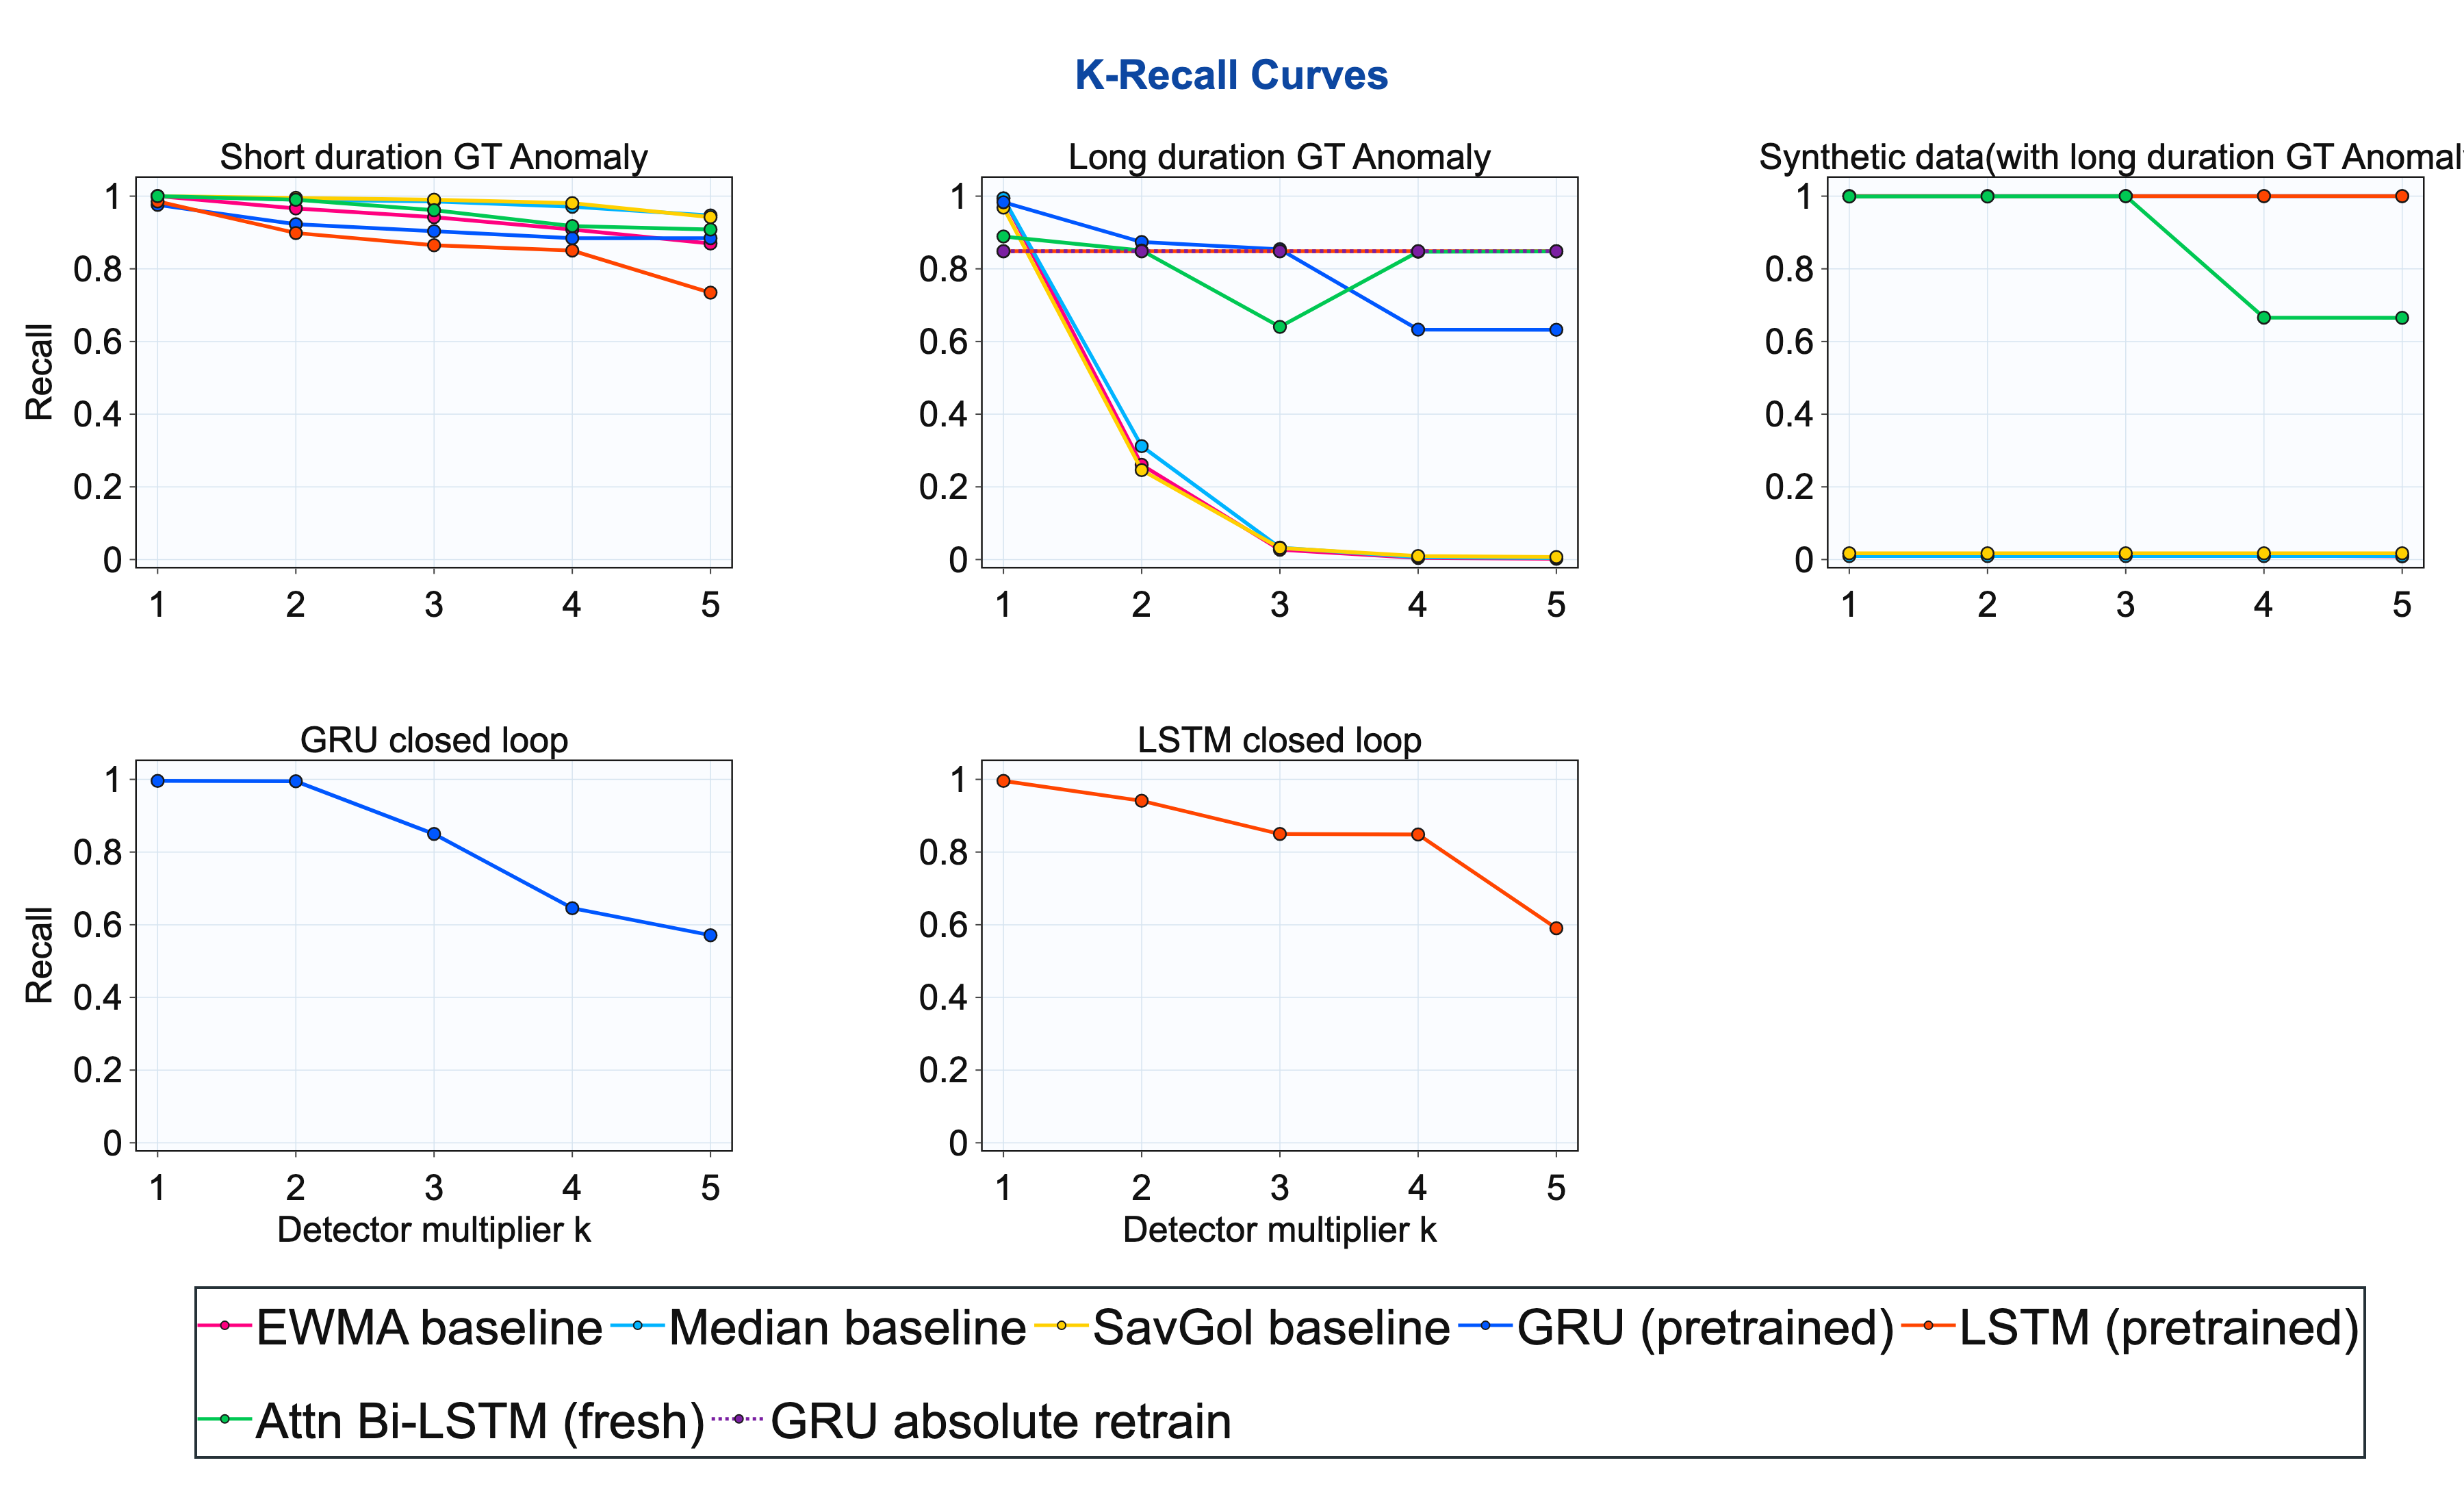
\includegraphics[width=\textwidth]{k_recall_curves_five_scenarios.png}
\caption{Recall versus detector multiplier $k$ for six schemes across five scenario panels (zero-historic benchmark).}
\label{fig:k_recall_five}
\end{figure}

\begin{figure}[htbp]
\centering
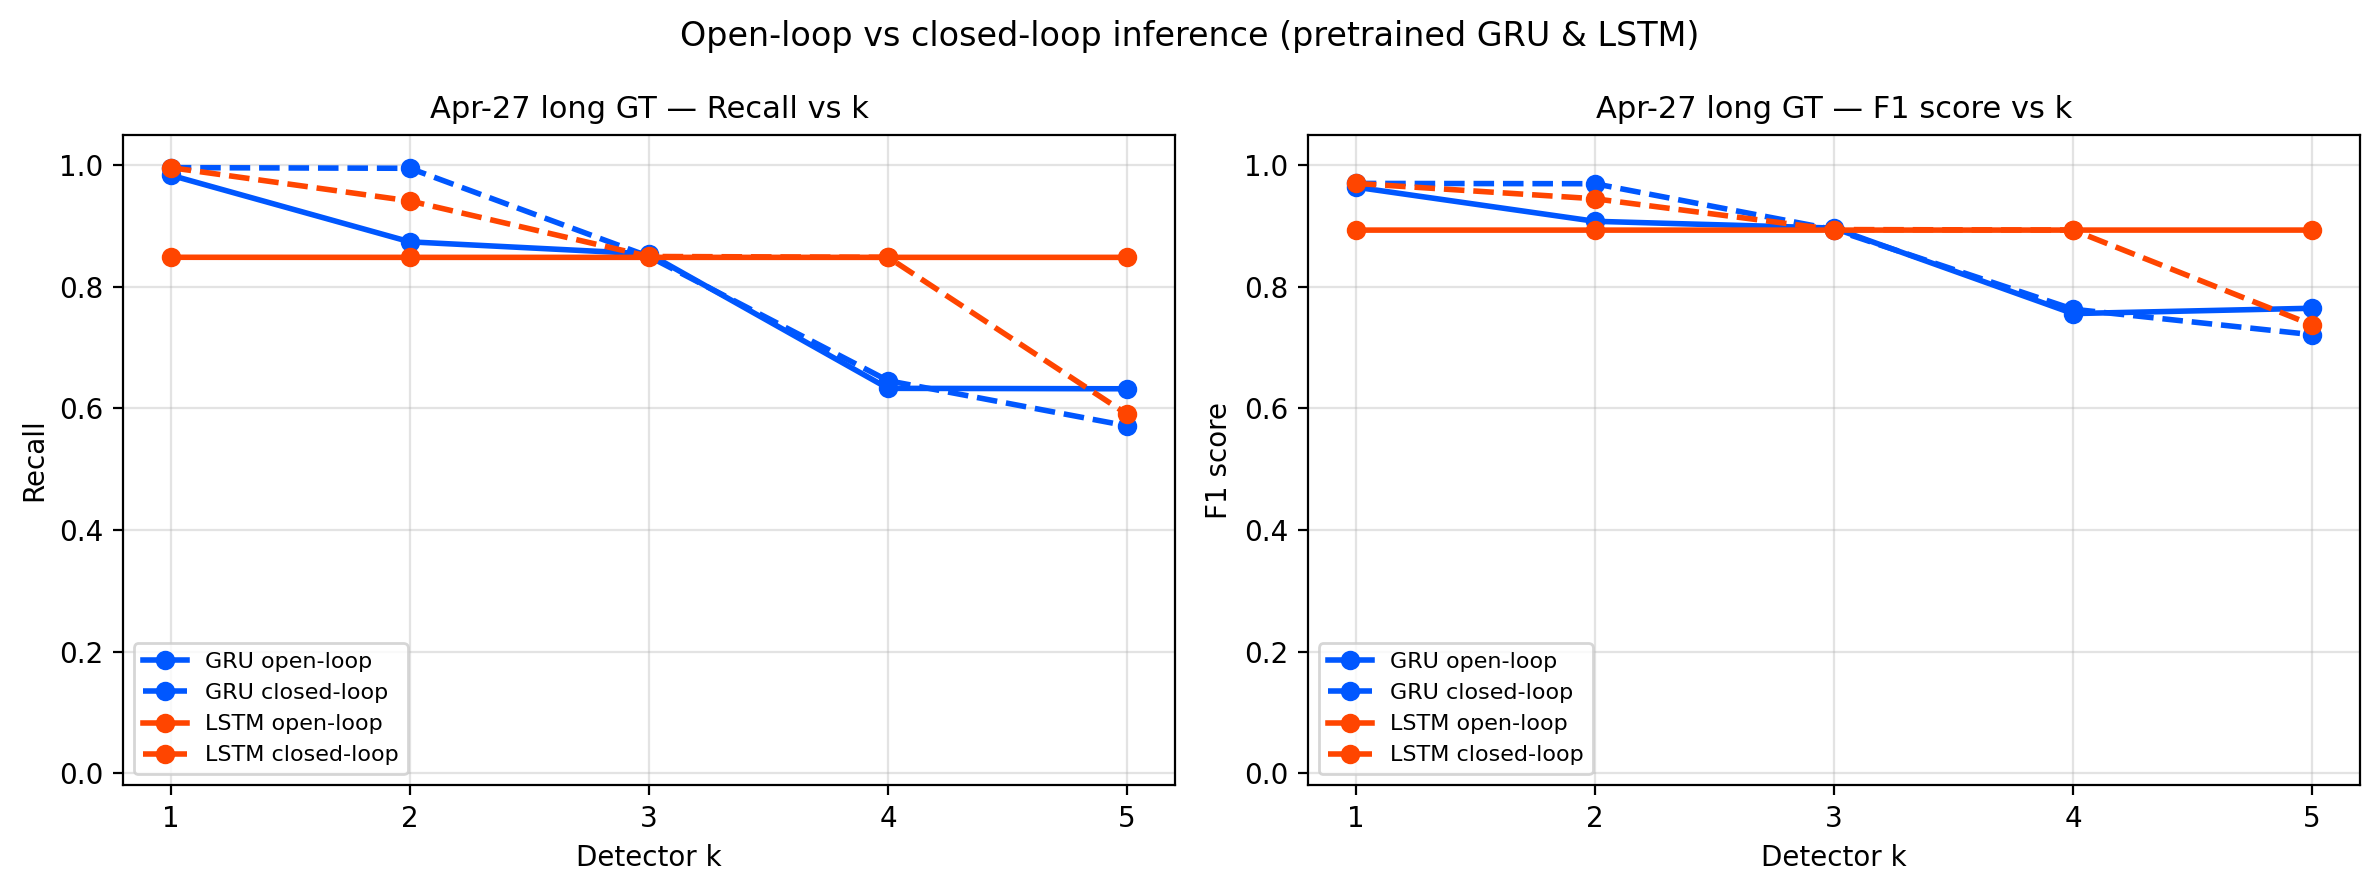
\includegraphics[width=0.85\textwidth]{k_recall_apr27_open_vs_closed_loop.png}
\caption{Apr-27 long ground truth: open-loop versus closed-loop GRU and LSTM at $k=4$.}
\label{fig:apr27_open_closed}
\end{figure}

\subsection{Mechanism for the GRU cliff}
When a predictor tracks a sustained level shift, the residual $|B-\hat B|$ shrinks in the interior of a long labelled interval. Raising $k$ raises the threshold; interior seconds then fall below the threshold even though the ground truth remains positive. LSTM checkpoints used here maintain larger interior residuals on Apr-27; GRU checkpoints track the plateau more tightly. A retraining ablation with absolute targets restores flat recall across $k$, confirming that the effect is linked to predictor behaviour rather than to the labelling file alone.

\subsection{Synthetic long-window layout}
With flat synthetic magnetics and long-window labels, GRU recall stays near 100\% for all $k$. The Apr-27 cliff therefore requires both the long label layout and realistic field shape during the event, not the label geometry alone.

\subsection{Deployment guidance}
For long campaigns with sustained anomalies, pretrained LSTM at $k \approx 3$ is the most stable choice in this study. GRU at $k \ge 4$ on long ground truth is not recommended without retraining or threshold tuning. Short campaigns may use $k=4$ with either recurrent model. Full point-level counts appear in Tables~\ref{tab:anomaly_k_recall_zero_hist_I} and~\ref{tab:anomaly_k_recall_zero_hist_II}.

% Requires: \usepackage{multirow}
% Model column: \multirow spans all scenario×k rows; scenario rules use
% \cline{2-12} so horizontal lines do not cut through the merged model cell.
\begin{table*}[t]
\centering
\footnotesize
\caption{Point-level anomaly detection across six schemes, three open-loop scenarios (short / long / synthetic GT), and GRU/LSTM closed-loop on Apr-27 long GT (\texttt{PREDICTOR\_AR\_CLOSED\_LOOP=1}), for $k \in \{1,\ldots,5\}$ (zero-historic, predict-only benchmark). Short Duration: 4{,}711 s; Long Duration: 8{,}825 s; Synthetic: 10{,}800 s. Part~I: EWMA, Median, Savitzky--Golay, and Attention Bi-LSTM.}
\label{tab:anomaly_k_recall_zero_hist_I}
\resizebox{\textwidth}{!}{
\begin{tabular}{|l|l|c|r|r|r|r|c|c|c|c|c|}
\hline
\textbf{Model} & \textbf{Scenario} & $\mathbf{K}$ & \textbf{TP} & \textbf{FP} & \textbf{TN} & \textbf{FN} & \textbf{Recall} & \textbf{Precision} & \textbf{F1} & \textbf{Specificity} & \textbf{Accuracy} \\
\hline
\multirow{15}{*}{EWMA} & \multirow{5}{*}{Short Duration Anomaly} & 1 & 207 & 4450 & 54 & 0 & 1.0000 & 0.0444 & 0.0851 & 0.0120 & 0.0554 \\
 &  & 2 & 200 & 1201 & 3303 & 7 & 0.9662 & 0.1428 & 0.2488 & 0.7333 & 0.7436 \\
 &  & 3 & 195 & 149 & 4355 & 12 & 0.9420 & 0.5669 & 0.7078 & 0.9669 & 0.9658 \\
 &  & 4 & 188 & 40 & 4464 & 19 & 0.9082 & 0.8246 & 0.8644 & 0.9911 & 0.9875 \\
 &  & 5 & 180 & 29 & 4475 & 27 & 0.8696 & 0.8612 & 0.8654 & 0.9936 & 0.9881 \\
\cline{2-12}
 & \multirow{5}{*}{Long Duration Anomaly} & 1 & 8293 & 481 & 0 & 51 & 0.9939 & 0.9452 & 0.9689 & 0.0000 & 0.9397 \\
 &  & 2 & 2174 & 90 & 391 & 6170 & 0.2605 & 0.9602 & 0.4099 & 0.8129 & 0.2907 \\
 &  & 3 & 225 & 44 & 437 & 8119 & 0.0270 & 0.8364 & 0.0522 & 0.9085 & 0.0750 \\
 &  & 4 & 39 & 36 & 445 & 8305 & 0.0047 & 0.5200 & 0.0093 & 0.9252 & 0.0548 \\
 &  & 5 & 19 & 34 & 447 & 8325 & 0.0023 & 0.3585 & 0.0045 & 0.9293 & 0.0528 \\
\cline{2-12}
 & \multirow{5}{*}{Synthetic Data} & 1 & 87 & 5366 & 31 & 5316 & 0.0161 & 0.0160 & 0.0160 & 0.0057 & 0.0109 \\
 &  & 2 & 75 & 4958 & 439 & 5328 & 0.0139 & 0.0149 & 0.0144 & 0.0813 & 0.0476 \\
 &  & 3 & 68 & 4525 & 872 & 5335 & 0.0126 & 0.0148 & 0.0136 & 0.1616 & 0.0870 \\
 &  & 4 & 63 & 4495 & 902 & 5340 & 0.0117 & 0.0138 & 0.0126 & 0.1671 & 0.0894 \\
 &  & 5 & 47 & 4302 & 1095 & 5356 & 0.0087 & 0.0108 & 0.0096 & 0.2029 & 0.1057 \\
\hline
\multirow{15}{*}{Median} & \multirow{5}{*}{Short Duration Anomaly} & 1 & 207 & 4453 & 51 & 0 & 1.0000 & 0.0444 & 0.0851 & 0.0113 & 0.0548 \\
 &  & 2 & 205 & 1576 & 2928 & 2 & 0.9903 & 0.1151 & 0.2062 & 0.6501 & 0.6650 \\
 &  & 3 & 204 & 231 & 4273 & 3 & 0.9855 & 0.4690 & 0.6355 & 0.9487 & 0.9503 \\
 &  & 4 & 201 & 71 & 4433 & 6 & 0.9710 & 0.7390 & 0.8392 & 0.9842 & 0.9837 \\
 &  & 5 & 196 & 46 & 4458 & 11 & 0.9469 & 0.8099 & 0.8731 & 0.9898 & 0.9879 \\
\cline{2-12}
 & \multirow{5}{*}{Long Duration Anomaly} & 1 & 8295 & 479 & 2 & 49 & 0.9941 & 0.9454 & 0.9692 & 0.0042 & 0.9402 \\
 &  & 2 & 2603 & 121 & 360 & 5741 & 0.3120 & 0.9556 & 0.4704 & 0.7484 & 0.3358 \\
 &  & 3 & 272 & 58 & 423 & 8072 & 0.0326 & 0.8242 & 0.0627 & 0.8794 & 0.0788 \\
 &  & 4 & 52 & 50 & 431 & 8292 & 0.0062 & 0.5098 & 0.0123 & 0.8960 & 0.0547 \\
 &  & 5 & 34 & 49 & 432 & 8310 & 0.0041 & 0.4096 & 0.0081 & 0.8981 & 0.0528 \\
\cline{2-12}
 & \multirow{5}{*}{Synthetic Data} & 1 & 51 & 5358 & 39 & 5352 & 0.0094 & 0.0094 & 0.0094 & 0.0072 & 0.0083 \\
 &  & 2 & 51 & 5045 & 352 & 5352 & 0.0094 & 0.0100 & 0.0097 & 0.0652 & 0.0373 \\
 &  & 3 & 51 & 4562 & 835 & 5352 & 0.0094 & 0.0111 & 0.0102 & 0.1547 & 0.0820 \\
 &  & 4 & 51 & 4503 & 894 & 5352 & 0.0094 & 0.0112 & 0.0102 & 0.1656 & 0.0875 \\
 &  & 5 & 51 & 4307 & 1090 & 5352 & 0.0094 & 0.0117 & 0.0104 & 0.2020 & 0.1056 \\
\hline
\multirow{15}{*}{Savitzky--Golay} & \multirow{5}{*}{Short Duration Anomaly} & 1 & 207 & 4324 & 180 & 0 & 1.0000 & 0.0457 & 0.0874 & 0.0400 & 0.0821 \\
 &  & 2 & 206 & 1142 & 3362 & 1 & 0.9952 & 0.1528 & 0.2650 & 0.7464 & 0.7574 \\
 &  & 3 & 205 & 184 & 4320 & 2 & 0.9903 & 0.5270 & 0.6879 & 0.9591 & 0.9605 \\
 &  & 4 & 203 & 77 & 4427 & 4 & 0.9807 & 0.7250 & 0.8337 & 0.9829 & 0.9828 \\
 &  & 5 & 195 & 52 & 4452 & 12 & 0.9420 & 0.7895 & 0.8590 & 0.9885 & 0.9864 \\
\cline{2-12}
 & \multirow{5}{*}{Long Duration Anomaly} & 1 & 8083 & 474 & 7 & 261 & 0.9687 & 0.9446 & 0.9565 & 0.0146 & 0.9167 \\
 &  & 2 & 2055 & 125 & 356 & 6289 & 0.2463 & 0.9427 & 0.3905 & 0.7401 & 0.2732 \\
 &  & 3 & 265 & 73 & 408 & 8079 & 0.0318 & 0.7840 & 0.0610 & 0.8482 & 0.0763 \\
 &  & 4 & 79 & 70 & 411 & 8265 & 0.0095 & 0.5302 & 0.0186 & 0.8545 & 0.0555 \\
 &  & 5 & 57 & 70 & 411 & 8287 & 0.0068 & 0.4488 & 0.0135 & 0.8545 & 0.0530 \\
\cline{2-12}
 & \multirow{5}{*}{Synthetic Data} & 1 & 93 & 5312 & 85 & 5310 & 0.0172 & 0.0172 & 0.0172 & 0.0157 & 0.0165 \\
 &  & 2 & 93 & 4834 & 563 & 5310 & 0.0172 & 0.0189 & 0.0180 & 0.1043 & 0.0607 \\
 &  & 3 & 93 & 4553 & 844 & 5310 & 0.0172 & 0.0200 & 0.0185 & 0.1564 & 0.0868 \\
 &  & 4 & 93 & 4508 & 889 & 5310 & 0.0172 & 0.0202 & 0.0186 & 0.1647 & 0.0909 \\
 &  & 5 & 93 & 4386 & 1011 & 5310 & 0.0172 & 0.0208 & 0.0188 & 0.1873 & 0.1022 \\
\hline
\multirow{15}{*}{Attention Bi-LSTM} & \multirow{5}{*}{Short Duration Anomaly} & 1 & 207 & 4322 & 182 & 0 & 1.0000 & 0.0457 & 0.0874 & 0.0404 & 0.0826 \\
 &  & 2 & 205 & 929 & 3575 & 2 & 0.9903 & 0.1808 & 0.3057 & 0.7937 & 0.8024 \\
 &  & 3 & 199 & 50 & 4454 & 8 & 0.9614 & 0.7992 & 0.8728 & 0.9889 & 0.9877 \\
 &  & 4 & 190 & 5 & 4499 & 17 & 0.9179 & 0.9744 & 0.9453 & 0.9989 & 0.9953 \\
 &  & 5 & 188 & 5 & 4499 & 19 & 0.9082 & 0.9741 & 0.9400 & 0.9989 & 0.9949 \\
\cline{2-12}
 & \multirow{5}{*}{Long Duration Anomaly} & 1 & 7419 & 476 & 5 & 925 & 0.8891 & 0.9397 & 0.9137 & 0.0104 & 0.8412 \\
 &  & 2 & 7096 & 425 & 56 & 1248 & 0.8504 & 0.9435 & 0.8945 & 0.1164 & 0.8104 \\
 &  & 3 & 5344 & 425 & 56 & 3000 & 0.6405 & 0.9263 & 0.7573 & 0.1164 & 0.6119 \\
 &  & 4 & 7066 & 421 & 60 & 1278 & 0.8468 & 0.9438 & 0.8927 & 0.1247 & 0.8075 \\
 &  & 5 & 7077 & 268 & 213 & 1267 & 0.8482 & 0.9635 & 0.9022 & 0.4428 & 0.8261 \\
\cline{2-12}
 & \multirow{5}{*}{Synthetic Data} & 1 & 5398 & 4676 & 721 & 5 & 0.9991 & 0.5358 & 0.6976 & 0.1336 & 0.5666 \\
 &  & 2 & 5398 & 4434 & 963 & 5 & 0.9991 & 0.5490 & 0.7086 & 0.1784 & 0.5890 \\
 &  & 3 & 5403 & 3157 & 2240 & 0 & 1.0000 & 0.6312 & 0.7739 & 0.4150 & 0.7077 \\
 &  & 4 & 3598 & 4497 & 900 & 1805 & 0.6659 & 0.4445 & 0.5331 & 0.1668 & 0.4165 \\
 &  & 5 & 3595 & 4495 & 902 & 1808 & 0.6654 & 0.4444 & 0.5329 & 0.1671 & 0.4164 \\
\hline
\end{tabular}
}
\end{table*}

\begin{table*}[p]
\centering
\footnotesize
\caption{Point-level anomaly detection across six schemes, three open-loop scenarios (short / long / synthetic GT), and GRU/LSTM closed-loop on Apr-27 long GT (\texttt{PREDICTOR\_AR\_CLOSED\_LOOP=1}), for $k \in \{1,\ldots,5\}$ (zero-historic, predict-only benchmark). Short Duration: 4{,}711 s; Long Duration: 8{,}825 s; Synthetic: 10{,}800 s. Part~II: GRU and LSTM (including Apr-27 closed-loop).}
\label{tab:anomaly_k_recall_zero_hist_II}
\resizebox{\textwidth}{!}{
\begin{tabular}{|l|l|c|r|r|r|r|c|c|c|c|c|}
\hline
\textbf{Model} & \textbf{Scenario} & $\mathbf{K}$ & \textbf{TP} & \textbf{FP} & \textbf{TN} & \textbf{FN} & \textbf{Recall} & \textbf{Precision} & \textbf{F1} & \textbf{Specificity} & \textbf{Accuracy} \\
\hline
\multirow{20}{*}{GRU} & \multirow{5}{*}{Short Duration Anomaly} & 1 & 202 & 3717 & 787 & 5 & 0.9758 & 0.0515 & 0.0979 & 0.1747 & 0.2099 \\
 &  & 2 & 191 & 1831 & 2673 & 16 & 0.9227 & 0.0945 & 0.1714 & 0.5935 & 0.6079 \\
 &  & 3 & 187 & 390 & 4114 & 20 & 0.9034 & 0.3241 & 0.4770 & 0.9134 & 0.9130 \\
 &  & 4 & 183 & 41 & 4463 & 24 & 0.8841 & 0.8170 & 0.8492 & 0.9909 & 0.9862 \\
 &  & 5 & 183 & 22 & 4482 & 24 & 0.8841 & 0.8927 & 0.8883 & 0.9951 & 0.9902 \\
\cline{2-12}
 & \multirow{5}{*}{Long Duration Anomaly} & 1 & 8205 & 479 & 2 & 139 & 0.9833 & 0.9448 & 0.9637 & 0.0042 & 0.9300 \\
 &  & 2 & 7291 & 432 & 49 & 1053 & 0.8738 & 0.9441 & 0.9076 & 0.1019 & 0.8317 \\
 &  & 3 & 7125 & 428 & 53 & 1219 & 0.8539 & 0.9433 & 0.8964 & 0.1102 & 0.8134 \\
 &  & 4 & 5281 & 349 & 132 & 3063 & 0.6329 & 0.9380 & 0.7558 & 0.2744 & 0.6134 \\
 &  & 5 & 5275 & 179 & 302 & 3069 & 0.6322 & 0.9672 & 0.7646 & 0.6279 & 0.6320 \\
\cline{2-12}
 & \multirow{5}{*}{Synthetic Data} & 1 & 5403 & 4571 & 826 & 0 & 1.0000 & 0.5417 & 0.7027 & 0.1530 & 0.5768 \\
 &  & 2 & 5403 & 4000 & 1397 & 0 & 1.0000 & 0.5746 & 0.7298 & 0.2588 & 0.6296 \\
 &  & 3 & 5403 & 3668 & 1729 & 0 & 1.0000 & 0.5956 & 0.7466 & 0.3204 & 0.6604 \\
 &  & 4 & 5403 & 2352 & 3045 & 0 & 1.0000 & 0.6967 & 0.8212 & 0.5642 & 0.7822 \\
 &  & 5 & 5403 & 1983 & 3414 & 0 & 1.0000 & 0.7315 & 0.8449 & 0.6326 & 0.8164 \\
\cline{2-12}
 & \multirow{5}{*}{GRU Closed-loop} & 1 & 8309 & 481 & 0 & 35 & 0.9958 & 0.9453 & 0.9699 & 0.0000 & 0.9415 \\
 &  & 2 & 8300 & 481 & 0 & 44 & 0.9947 & 0.9452 & 0.9693 & 0.0000 & 0.9405 \\
 &  & 3 & 7090 & 428 & 53 & 1254 & 0.8497 & 0.9431 & 0.8940 & 0.1102 & 0.8094 \\
 &  & 4 & 5386 & 388 & 93 & 2958 & 0.6455 & 0.9328 & 0.7630 & 0.1933 & 0.6208 \\
 &  & 5 & 4766 & 108 & 373 & 3578 & 0.5712 & 0.9778 & 0.7211 & 0.7755 & 0.5823 \\
\hline
\multirow{20}{*}{LSTM} & \multirow{5}{*}{Short Duration Anomaly} & 1 & 204 & 3804 & 700 & 3 & 0.9855 & 0.0509 & 0.0968 & 0.1554 & 0.1919 \\
 &  & 2 & 186 & 936 & 3568 & 21 & 0.8986 & 0.1658 & 0.2799 & 0.7922 & 0.7969 \\
 &  & 3 & 179 & 58 & 4446 & 28 & 0.8647 & 0.7553 & 0.8063 & 0.9871 & 0.9817 \\
 &  & 4 & 176 & 15 & 4489 & 31 & 0.8502 & 0.9215 & 0.8844 & 0.9967 & 0.9902 \\
 &  & 5 & 152 & 12 & 4492 & 55 & 0.7343 & 0.9268 & 0.8194 & 0.9973 & 0.9858 \\
\cline{2-12}
 & \multirow{5}{*}{Long Duration Anomaly} & 1 & 7079 & 430 & 51 & 1265 & 0.8484 & 0.9427 & 0.8931 & 0.1060 & 0.8079 \\
 &  & 2 & 7078 & 429 & 52 & 1266 & 0.8483 & 0.9429 & 0.8931 & 0.1081 & 0.8079 \\
 &  & 3 & 7078 & 429 & 52 & 1266 & 0.8483 & 0.9429 & 0.8931 & 0.1081 & 0.8079 \\
 &  & 4 & 7078 & 428 & 53 & 1266 & 0.8483 & 0.9430 & 0.8931 & 0.1102 & 0.8080 \\
 &  & 5 & 7078 & 428 & 53 & 1266 & 0.8483 & 0.9430 & 0.8931 & 0.1102 & 0.8080 \\
\cline{2-12}
 & \multirow{5}{*}{Synthetic Data} & 1 & 5403 & 4591 & 806 & 0 & 1.0000 & 0.5406 & 0.7018 & 0.1493 & 0.5749 \\
 &  & 2 & 5403 & 3877 & 1520 & 0 & 1.0000 & 0.5822 & 0.7360 & 0.2816 & 0.6410 \\
 &  & 3 & 5403 & 2392 & 3005 & 0 & 1.0000 & 0.6931 & 0.8188 & 0.5568 & 0.7785 \\
 &  & 4 & 5403 & 701 & 4696 & 0 & 1.0000 & 0.8852 & 0.9391 & 0.8701 & 0.9351 \\
 &  & 5 & 5403 & 88 & 5309 & 0 & 1.0000 & 0.9840 & 0.9919 & 0.9837 & 0.9919 \\
\cline{2-12}
 & \multirow{5}{*}{LSTM Closed-loop} & 1 & 8309 & 481 & 0 & 35 & 0.9958 & 0.9453 & 0.9699 & 0.0000 & 0.9415 \\
 &  & 2 & 7852 & 429 & 52 & 492 & 0.9410 & 0.9482 & 0.9446 & 0.1081 & 0.8956 \\
 &  & 3 & 7090 & 428 & 53 & 1254 & 0.8497 & 0.9431 & 0.8940 & 0.1102 & 0.8094 \\
 &  & 4 & 7079 & 428 & 53 & 1265 & 0.8484 & 0.9430 & 0.8932 & 0.1102 & 0.8082 \\
 &  & 5 & 4925 & 92 & 389 & 3419 & 0.5902 & 0.9817 & 0.7372 & 0.8087 & 0.6022 \\
\hline
\end{tabular}
}
\end{table*}
% 100 data cells (60 + 40)


\section{Direction of the Magnetic Perturbation}
When CSV or database rows provide three orthogonal components, the application subtracts a quiet-period baseline (median per component) and forms the perturbation vector $\Delta\mathbf{B}$. Azimuth and inclination follow standard spherical conventions; a unit vector is drawn in the 3D panel. If two observatories flag anomalies within a short interval, bearing lines can be intersected for a rough source location.

This step estimates the direction of $\Delta\mathbf{B}$, not necessarily the bearing to a compact source. Near-field geometry, baseline drift, and timing mismatch between components can bias the result. Chapter~\ref{Chapter7} lists improvements such as calibration runs and dipole inversion.

\section*{Summary}
Recurrent predictors outperform direct smoothing on long-duration ground truth. LSTM is more stable across threshold settings; GRU shows a sharp recall drop at $k \ge 4$ on Apr-27 because of tight plateau tracking. The benchmark scripts and result tables in the repository allow independent reproduction of these figures.

% Chapter 6
\chapter{Visualization and User Interface}
\label{Chapter6}
\lhead{Chapter 6. \emph{Visualization and User Interface}}

This chapter describes the visualisation and user interface of Magnavis, with emphasis on the DB-backed multi-sensor variant (application\_temp.py).

\section{Time-Series Plots}
Each selected sensor has a dedicated panel in the left half of the window. The plot shows \textbf{B (nT)} --- the low-pass filtered resultant magnetic field magnitude over time. Real-time (or simulation/CSV) data are appended as they arrive. Predicted values are overlaid when \texttt{predict\_out.csv} is available. Anomalies are drawn as vertical lines on the time-series axes, allowing quick visual correlation of flagged times with the signal.

\section{Shared Parameters Panel}
A single control panel on the right applies to all sensors:
\begin{itemize}
    \item \textbf{Anomaly threshold multiplier:} Controls sensitivity of anomaly detection (higher = stricter).
    \item \textbf{Training window (minutes):} Restricts predictor training to the most recent N minutes; 0 means full history. Passed to the subprocess via \texttt{TRAIN\_WINDOW\_MINUTES}.
    \item \textbf{Anomaly freeze window (minutes):} Duration for which the threshold is frozen after the first anomaly.
\end{itemize}
Changes are synced to all sensor contexts and to all registered control widgets so that each panel reflects the same values.

\section{3D Anomaly Direction Plot}
The 3D plot uses Matplotlib's \texttt{projection="3d"}. The origin represents the observatory centre; axes typically correspond to East, North, and Up (or sensor-frame axes). Each recorded anomaly direction (azimuth, inclination) is converted to a unit vector $(u, v, w)$ and drawn as a quiver from $(0,0,0)$ to $(u,v,w)$. OBS1 and OBS2 can be distinguished by colour (e.g. blue and orange); the last 30 directions are shown, with older ones optionally faded. The latest anomaly direction is highlighted (e.g. red arrow). When no direction data are available, a placeholder (e.g. ``---'') can be displayed.

\section{Log and Status}
The log area displays application messages (info, warning, error). Each anomaly can be logged with timestamp, sensor, magnitude, and (for OBS1/OBS2 in CSV mode) direction details (azimuth, inclination, $|\Delta B|$). A status line above the log can show the latest anomaly direction and current threshold.

\section{Offline and CSV Modes}
In CSV mode, the user selects a CSV file containing time-series and optionally component data. Direction finding is available when all three components for an observatory (e.g. OBS1\_1, OBS1\_2, OBS1\_3) are present. In simulation mode, the clock advances and data are fetched from the DB for the selected sensors; in real-time mode, the latest historic window is polled periodically.

\section{Session Layout}
Session output is organised under \texttt{sessions/<session\_id>/}. In the multi-sensor variant, each sensor has a subfolder \texttt{<sensor\_id>/} containing \texttt{predict\_input.csv}, \texttt{predict\_out.csv}, \texttt{predict\_stdout.log}, and \texttt{predict\_stderr.log}. This allows per-sensor inspection and debugging.

\section*{Summary}
Visualisation in Magnavis centres on time-series plots of the filtered resultant B (nT), overlaid predictions and anomaly markers, and a 3D direction plot for anomaly bearings. The shared parameters panel and scrollable log support multi-sensor operation without cluttering the UI. The design supports real-time, simulation, and CSV workflows with consistent behaviour across modes.

% Chapter 7
\chapter{Conclusion and Future Work}
\label{Chapter7}
\lhead{Chapter 7. \emph{Conclusion and Future Work}}

\section{Conclusion}
This thesis presented Magnavis, a software framework for magnetic observatory data that links ingestion, recurrent forecasting, residual-based anomaly detection, and optional perturbation-direction visualisation. The main scientific contribution of the current work is a controlled benchmark under zero-historic, predict-only operation, comparing statistical smoothers, a session-trained attention bidirectional LSTM, and pretrained GRU and LSTM models on short, long, and synthetic ground-truth layouts.

Three conclusions follow from the experiments. First, detector multiplier $k$ must be chosen together with the predictor: on long-duration ground truth, offline smoothers fail at moderate $k$, whereas neural predictors can remain useful. Second, pretrained LSTM delivers roughly flat 85\% recall on Apr-27 for $k=2$--$5$; pretrained GRU matches LSTM at $k=3$ but falls to about 63\% for $k \ge 4$ because interior residuals shrink when the model tracks a sustained offset. Closed-loop autoregressive rolling does not remove that gap. Third, for operational use on long campaigns, LSTM at $k \approx 3$ is the most robust setting identified here; GRU at high $k$ on long ground truth requires retraining or careful validation.

The direction-finding module provides a geometric characterisation of tri-axial perturbations and optional two-station triangulation. Field experience shows that reported bearings may disagree with known source positions unless baselines, alignment, and timing are carefully controlled.

\section{Limitations}
\begin{itemize}
    \item Point-level metrics on fixed CSV exports may not capture event-level detection delay or operator workflow in live mode.
    \item Pretrained weights reflect a specific training archive and sensor; transfer to other sites is not guaranteed.
    \item Direction finding reports the perturbation vector, not a unique source location.
    \item Database credentials and session logs in the prototype should be externalised before production deployment.
\end{itemize}

\section{Future Work}
\begin{enumerate}[label=(\alph*)]
    \item Event-level recall and detection latency on manual anomaly intervals.
    \item Systematic GRU retraining studies (absolute versus delta targets) and checkpoint selection criteria.
    \item Calibration of direction estimates using controlled source runs at known bearings.
    \item Dipole or multi-point inversion using vector anomalies at two observatories.
    \item Extension of the benchmark to additional OBS sensors and months of archive data.
    \item Integration of the evaluation harness into continuous integration for regression testing after model updates.
\end{enumerate}

\section{Closing Remarks}
Magnavis demonstrates that a single open pipeline can support both interactive monitoring and rigorous offline comparison of forecasting and detection choices. The repository, bundled models, and benchmark summaries provide a reproducible basis for thesis examination and for further research on static observatory magnetic anomaly detection at IIT Kanpur.


%----------------------------------------------------------------------------------------
%	APPENDICES
%----------------------------------------------------------------------------------------
\addtocontents{toc}{\vspace{2em}}
\appendix
\chapter{Benchmark Reproduction Notes}\doublespacing
\label{AppendixA}
\lhead{Appendix A. \emph{Benchmark Reproduction}}

This appendix lists commands to reproduce the main $k$--recall evaluation from the Magnavis repository.

\section{Environment}
Create a Python virtual environment and install dependencies from \texttt{requirements\_feb\_2025.txt}. Place labelled CSV files in \texttt{Datafiles/} as described in \texttt{Datafiles/README.md}.

\section{Run}
\begin{verbatim}
cd src/benchmark_feb13_2026_improved
python run_k_recall_curves.py
\end{verbatim}

Results are written under \texttt{results/k\_recall\_curves\_<timestamp>/}, including \texttt{k\_recall\_points.csv} and figure PNG files.

\section{Key Environment Variables}
\begin{itemize}
    \item \texttt{MAGNAVIS\_BATCH\_HISTORIC\_MINUTES=0} --- zero-historic protocol.
    \item \texttt{PREDICTOR\_MODEL\_FAMILY} --- \texttt{gru} or \texttt{lstm}.
    \item \texttt{PREDICTOR\_AR\_CLOSED\_LOOP=1} --- closed-loop runs on Apr-27.
\end{itemize}

\addtocontents{toc}{\vspace{2em}}

\backmatter
%----------------------------------------------------------------------------------------
%	BIBLIOGRAPHY
%----------------------------------------------------------------------------------------
\nocite{*}
\label{Bibliography}
\lhead{\emph{Bibliography}}
\bibliographystyle{ieeetr}
\bibliography{Bibliography}

\end{document}
